% !TeX spellcheck = de_DE
\chapter{Software}

\section{Einleitung und Überblick}
Die Softwareseite dieses Projekts umfasst das Programmieren eines Algorithmus in Matlab/Simulink, der für alle Berechnungen der Kinematik des 6-DOF-Roboterarms zuständig ist. Dieser Algorithmus wird mithilfe des Simulink Embedded Coders in C-Code generiert und danach auf einem STM32 Mikroprozessor ausgeführt. Die Datenübertragung vom Mikroprozessor zu den Motortreibern, die die Motoren betreiben, erfolgt über das Busprotokoll SPI. Encoder-Feedback wird zur Positionsregelung in die Regelschleife zurückgeführt.

Die Struktur unserer Softwarelösung ist wievolgt:\par
\par

\begin{figure}[h]
	\centering
	\vspace{-10pt}
	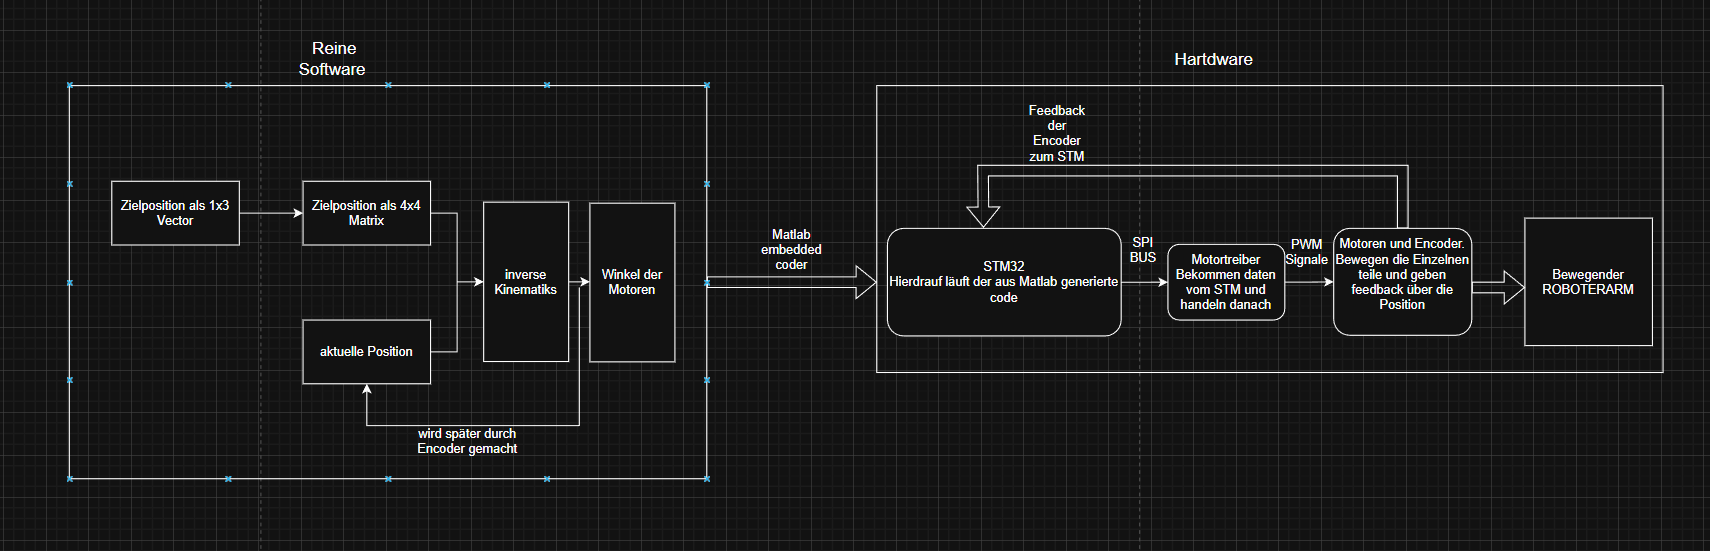
\includegraphics[width=1\textwidth]{figures/allgemein/roboterarm_flowchart.png}
	\caption{Struktur der Software}
	\label{fig:Softwarestruktur}
\end{figure}
% TODO neues bild einfügen sobald die struktur Fertig ist.

%\subsection{Aufgabenstellung}
%Da die Entwicklung unseres 6dof Roboterarms im Rahmen des Faches ASIT erfolgt und der Lernerfolg im Vordergrund steht konnten wir uns die Aufgabenstellung selbst Stellen und hatten dabei keine großen Einschränkungen.  Wir haben uns dazu entschieden das der Roboterarm als Mindestanforderung eine Pick and Place Operation, also ein Objekt aufheben und wo anders Platzieren können soll. Als Optionale weitere Herausforderung soll man über ein Graphical user Interface Koordinaten eingeben können zu denen sich der Arm dann bewegt.

\subsection{Toolchain}
% - Matlab/Simulink Version
% - Simulink Embedded Coder
% - STM32CubeIDE oder Keil
% - Workflow: Simulink → Code-Generierung → STM32
Die Entwicklung der Software erfolgt modellbasiert, zuerst wird ein Algorithmus in Simulink realisiert und getestet und danach mithilfe des in Simulink integrierten Embedded coders auf reale Hardware gebracht. Die Struktur ist in Abbildung \ref{fig:Softwarestruktur} beschrieben.

\subsubsection{Matlab and Simulink}
Matlab/Simulink r2025a dient als Grundlage für die Algorithmusentwicklung. Die Grafische auf Blöcken basierende Programmiersprache ermöglicht eine Intuitive Programmentwicklung, Kombiniert mit der Robotic systems Toolbox\cite{_2026_robotics} und Simscape\cite{a2026_simscape} ist ein sehr angenehmes Softwareentwickeln möglich.

Vorteile der modellbasierten Entwicklung mit Simulink:
\begin{itemize}
	\item \textbf{Simulation vor Hardware-Test}: Algorithmen können ohne 
	physische Hardware getestet werden
	\item \textbf{Grafische Darstellung}: Blockdiagramme visualisieren 
	Datenfluss und Abhängigkeiten und sind besser verständlich als Textbasiertes Programmieren
	\item \textbf{Integrierte Testumgebung}: Simulink bietet umfangreiche 
	Möglichkeiten für Unit-Tests und Verifikation
	\item \textbf{Lernerfolg}: Simulink ist in der Industrie weit verbreitet und als Elektrotechniker wichtig zu können
\end{itemize} 

% TODO: Entwicklungsumgebung beschreiben cube ide sobald wir das haben
% TODO: Etwas zu embedded coder einfügen sobald ich das habe
\newpage
\subsubsection{Workflow}

Der typische Entwicklungs-Workflow sieht wie folgt aus:

\begin{enumerate}
	\item \textbf{Modellierung}: Algorithmus in Simulink entwickeln
	\item \textbf{Simulation}: Funktionalität in Simulink via Simscape testen
	\item \textbf{Verifikation}: Korrektes Verhalten testen
	\item \textbf{Code-Generierung}: C-Code mit Embedded Coder erzeugen
	\item \textbf{Integration}: Code in STM32CubeIDE-Projekt einbinden
	\item \textbf{Kompilierung}: Projekt bauen und auf Fehler prüfen
	\item \textbf{Deployment}: Firmware auf STM32 flashen
	\item \textbf{Hardware-Test}: Funktionstest am realen Roboterarm
	\item \textbf{Iteration}: Bei Bedarf zurück zu Schritt 1
\end{enumerate}

Dieser Prozess ermöglicht eine schnelle Fehlersuche, da Probleme 
bereits in der Simulation erkannt werden können, bevor Hardware-Tests 
durchgeführt werden.

\subsection{Schnittstellen zur Hardware}
% TODO: Kurze Übersicht über Hardware-Schnittstellen
% - SPI-Kommunikation zu Motortreibern
% - Encoder-Feedback (Protokoll/Interface)
% - Signale für Motoransteuerung
% - Verweis auf Hardware-Kapitel für Details
\subsubsection{SPI-Bus}


\subsubsection{Signale zu den Motoren}

%%\section{Kinematik-Algorithmen}
%
%\subsection{Vorwärtskinematik}
%% TODO: Vorwärtskinematik beschreiben
%% - Berechnung der End-Effektor-Position aus Gelenkwinkeln
%% - Mathematische Grundlagen (DH-Parameter oder andere Methode)
%% - Implementierung in Simulink
%
%Die Vorwärtskinematik berechnet die Position und Orientierung des End-Effektors aus den gegebenen Gelenkwinkeln $\theta_1, \theta_2, ..., \theta_6$.
%
%\subsection{Inverse Kinematik}
%% TODO: Inverse Kinematik beschreiben
%% - Berechnung der Gelenkwinkel aus Zielposition (x,y,z)
%% - Lösungsansatz (analytisch/numerisch/geometrisch)
%% - Herausforderungen (Mehrdeutigkeit, Singularitäten)
%% - Implementierung in Simulink
%
%Die inverse Kinematik löst das Problem, aus einer gewünschten End-Effektor-Position die notwendigen Gelenkwinkel zu berechnen.
%
%\subsection{Transformationsmatrizen}
%% TODO: Transformationen beschreiben
%% - Koordinatensysteme und Frames
%% - Homogene Transformationsmatrizen (4x4)
%% - Umwandlung von 1x3 Positionsvektor zu 4x4 Matrix
%% - Rotation und Translation
%
%Die Transformation von einem 1x3 Positionsvektor zu einer 4x4 homogenen Transformationsmatrix ermöglicht die einheitliche Behandlung von Rotation und Translation.
%
%\[
%T = \begin{bmatrix}
%	R_{3\times3} & p_{3\times1} \\
%	0_{1\times3} & 1
%\end{bmatrix}
%\]
%
\section{Simulink-Modell}

\subsection{Modellarchitektur}
% TODO: Gesamtarchitektur des Simulink-Modells
% - Blockdiagramm einfügen (Ihr Bild aus der Frage!)
% - Übersicht über Hauptkomponenten
% - Datenfluss von Input zu Output

\begin{figure}[h]
	\centering
	% \includegraphics[width=\textwidth]{pfad/zu/ihrem/blockdiagramm.png}
	\caption{Softwarearchitektur des 6-DOF-Roboterarms}
	\label{fig:software_architektur}
\end{figure}

\subsection{Hauptblöcke und Subsysteme}

\subsubsection{Eingabe: Zielposition}
% TODO: Input-Schnittstelle beschreiben
% - Format der Zielposition (1x3 Vektor)
% - Koordinatensystem
% - Sollwert-Generierung

\subsubsection{Inverse Kinematik Block}
% TODO: IK-Block in Simulink
% - Implementierung des IK-Algorithmus
% - Input/Output-Schnittstellen
% - Embedded Matlab Function oder andere Blöcke

\subsubsection{Winkelberechnung für Motoren}
% TODO: Motorwinkel-Berechnung
% - Umrechnung von Gelenkwinkeln zu Motoransteuerung
% - Getriebe-Übersetzung (falls vorhanden)
% - Winkel-Normalisierung

\subsubsection{Feedback-Loop mit Encoder-Daten}
% TODO: Regelkreis beschreiben
% - Encoder-Feedback Integration
% - Differenz Soll-/Ist-Position
% - Regelungsalgorithmus (PID oder andere)
% - Closed-Loop Struktur

\subsection{Simulation und Validierung}
% TODO: Simulationsergebnisse
% - Test-Szenarien in Matlab
% - Simulationsergebnisse (Grafiken einfügen!)
% - Validierung der Kinematik
% - Performance-Analyse

\begin{figure}[h]
	\centering
	% \includegraphics[width=0.8\textwidth]{pfad/zu/simulation_ergebnis.png}
	\caption{Simulationsergebnis: Gelenkwinkel über Zeit}
	\label{fig:simulation}
\end{figure}

\section{Codegenerierung und STM32-Integration}

\subsection{Embedded Coder Konfiguration}
% TODO: Embedded Coder Setup
% - Target Hardware: STM32 (spezifisches Modell)
% - Compiler-Einstellungen
% - Optimierungsoptionen (Speed vs. RAM)
% - Code-Interface-Konfiguration
\begin{comment}
	Inhalt...

\subsection{Generierter C-Code}
% TODO: C-Code Analyse
% - Struktur des generierten Codes
% - Code-Beispiel (Ausschnitt 10-20 Zeilen)
% - Lesbarkeit und Wartbarkeit
% - Speicherbedarf

\begin{lstlisting}[language=C, caption={Beispiel: Generierter C-Code für Kinematik-Berechnung}]
	void inverse_kinematics_step(void) {
		// Berechnung der inversen Kinematik
		// Automatisch generiert aus Simulink-Modell
		...
	}
\end{lstlisting}

\subsection{Integration in STM32-Projekt}
% TODO: Integration beschreiben
% - Projektstruktur im STM32-Projekt
% - Einbindung in main.c
% - Initialisierung der generierten Funktionen
% - Interface zu HAL-Bibliotheken

\subsection{Haupt-Regelschleife und Timing}
% TODO: Echtzeitaspekte
% - Main-Loop Struktur
% - Zykluszeit (z.B. 1ms, 10ms, ...)
% - Timer-Konfiguration
% - Task-Scheduling
% - Interrupt-Handling

\subsection{Speicher- und Performance-Optimierung}
% TODO: Optimierungen
% - RAM/Flash-Nutzung
% - Berechnungszeit pro Zyklus
% - Profiling-Ergebnisse
% - Optimierungsmaßnahmen

\section{Sicherheit und Fehlerbehandlung}

\subsection{Software-Limitierung}
% TODO: Software-Limits beschreiben
% - Gelenkwinkel-Grenzen (min/max für jeden Joint)
% - Geschwindigkeitsbegrenzung
% - Beschleunigungslimits
% - Workspace-Begrenzung

\subsection{Fehlerbehandlung}
% TODO: Error-Handling
% - Unreachable Positions (IK hat keine Lösung)
% - Singularitäten erkennen und vermeiden
% - Numerische Stabilität
% - Fehler-Rückgabewerte

\subsection{Watchdog und Timeout}
% TODO: System-Sicherheit
% - Watchdog-Timer Konfiguration
% - Timeout-Mechanismen
% - Error-Recovery-Strategien
% - Safe-State bei Fehler

\section{Test und aktueller Stand}

\subsection{Matlab-Simulation}
% TODO: Simulations-Tests
% - Test-Szenarien (verschiedene Zielpositionen)
% - Ergebnisse (Grafiken einfügen!)
% - Validierung der Algorithmen
% - Performance in Simulation

\subsection{Tests auf STM32}
% TODO: Hardware-Tests (falls durchgeführt)
% - Testaufbau
% - Erste Tests auf echter Hardware
% - Beobachtungen und Messungen
% - Probleme und Lösungen

\subsection{Offene Punkte und nächste Schritte}
% TODO: Was fehlt noch?
% - Integration mit kompletter Hardware
% - Kalibrierung
% - Feintuning der Parameter
% - Optimierungen
% - Geplante Erweiterungen

\section{Fazit und Ausblick}

\subsection{Erreichte Funktionalität}
% TODO: Was funktioniert bereits?
% - Kinematik-Algorithmen validiert
% - Code-Generierung erfolgreich
% - Simulation liefert plausible Ergebnisse
% - Erste Tests auf STM32 (falls gemacht)

\subsection{Herausforderungen und Lösungen}
% TODO: Schwierigkeiten im Projekt
% - Technische Herausforderungen
% - Wie wurden sie gelöst?
% - Lessons Learned

\subsection{Ausblick}
% TODO: Nächste Schritte bis Projektende
% - Hardware-Software-Integration
% - Systemtests
% - Optimierungen
% - Mögliche Erweiterungen (Bahnplanung, Kollisionsvermeidung, ...)
\end{comment}